\documentclass[11pt]{article}  
\usepackage{kosemnet,ko-math,ngerman,enumitem}  
\setlist{noitemsep}

\author{Hans-Gert Gräbe, Leipzig}
\title{Reguläre Polyeder\kosemnetlicensemark}
\date{Version vom 11. Oktober 2021}

\begin{document}

\maketitle

\section*{Reguläre Polyeder}

Als \emph{konvexes Polyeder} bezeichnet man einen durch endlich viele ebene
Flä\-chen begrenzten Körper, wo zusammen mit je zwei Punkten auch alle Punkte
der Verbindungsstrecke zu diesem Körper gehören.

Jede Seitenfläche definiert eine Ebene, die \emph{Stützebene} des Polyeders zu
dieser Seitenfläche, so dass das Polyeder vollständig in einem Halbraum
bzgl.\ dieser Ebene liegt. Das Polyeder ist als Punktmenge genau der
Durchschnitt all dieser Halbräume. 

Wir beschränken uns im Weiteren auf beschränkte konvexe Polyeder, das sind
solche mit endlichem Volumen. 

Als \emph{reguläres Polyeder} bezeichnet man ein solches beschränktes konvexes
Polyeder, dessen Seitenflächen alle zueinander kongruente regelmäßige Vielecke
($q$-Ecke) sind \emph{und} in jeder Ecke die gleich Anzahl $p$ von Kanten
zusammenstößt.

Bekanntlich gibt es fünf solche Körper.
\begin{center}
  \includegraphics[width=.8\textwidth]{graebe-05-1/PlatonischeKoerper.jpg}\\
  \emph{Abbildung 1:} Die Platonischen Körper.\\ Quelle: Webseite von
  Carl-Friedrich Bödigheimer, Bonn. 
\end{center}
Dies war bereits in der Antike bekannt, weshalb diese Körper auch als
\textbf{Platonische Körper} bezeichnet werden.  

Dass reguläre Polyeder nur aus regelmäßigen Dreiecken, Vierecken oder
Fünfecken aufgebaut sein können, überlegt man sich zunächst leicht am lokalen
Aufbau möglicher Körpernetze, siehe Abbildung 2.

\begin{center}
  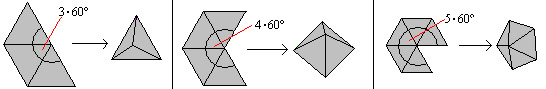
\includegraphics[width=.8\textwidth]{graebe-05-1/winkel-1.jpg}\\
  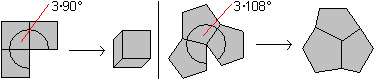
\includegraphics[width=.6\textwidth]{graebe-05-1/winkel-2.jpg}\\
  \emph{Abbildung 2:} Warum nur Dreiecke, Vierecke oder Fünfecke.\\ Quelle:
  Jürgen Köller. Mathematische Basteleien. \cite{KoellerPlatonisch}
\end{center}

\section*{Die Platonischen Körper erkunden}

Wie viele Ecken, Kanten und Flächen?
\begin{center}
  \begin{tabular}{|cc|ccc|l|}\hline
    $p$ & $q$ & $e$ & $k$ & $f$ & Name des Polyeders \\\hline
    3 & 3 &  4 &  6 &  4 & Tetraeder\\
    3 & 4 &  8 & 12 &  6 & Würfel (Hexaeder)\\
    4 & 3 &  6 & 12 &  8 & Oktaeder\\
    3 & 5 & 20 & 30 & 12 & Dodekaeder\\
    5 & 3 & 12 & 30 & 20 & Ikosaeder\\\hline
  \end{tabular}
\end{center}

\subsection*{Dualität}

$e_W=f_O$ und $e_O=f_W$ ist kein Zufall. Die Mittelpunkte der Seitenflächen
eines Würfels spannen ein Oktaeder auf, die Mittelpunkte der Seitenflächen
eines Oktaeders einen Würfel.

Ähnlich Dodekaeder und Ikosaeder.

Was aber ist mit dem Tetraeder? 

\subsection*{Symmetriegruppen}

Reguläre Polyeder haben eine sehr symmetrische Gestalt und lassen damit viele
räumliche Bewegungen zu, die das Polyeder in sich überführen. Wir wollen alle
herausfinden.  

\textbf{Tetraeder:} Jede der vier Seitenflächen kann nach unten gedreht
werden, und das in jeweils 3 Lagen. Also gibt es 12 Symmetriebewegungen.
Welche?

Dieselbe Frage für die anderen Platonischen Körper.

\subsection*{Größenverhältnisse}

Alle fünf Platonischen Körper haben eine Umkugel und eine Inkugel, deren
Mittelpunkt jeweils im Zentrum $Z$ des Körpers liegt. Um Größenverhältnisse zu
vergleichen, wollen wir für den Radius der Umkugel $R=1$ annehmen und jeweils
Kantenlänge $a$, Oberfläche $O$, Volumen $V$ und Inkugelradius $r$ bestimmen
und mit den entsprechenden Größen $O=4\pi\approx 12.57$ und $V=\frac43\pi
\approx 4.189$ der Umkugel vergleichen. 

Dabei wollen wir geeignete Schnitte durch die jeweilige räumliche Figur legen,
in denen wir die uns interessierenden Größenverhältnisse in einer ebenen Figur
wiederfinden, und dann Ansätze der ebenen Geometrie zur Anwendung bringen.

\paragraph{Tetraeder.}
Lege eine Ebene durch eine Kante und $Z$. Die Schnittfigur ist ein
gleichschenkliges Dreieck mit der Basislänge $a$ und den Schenkellängen $h$ --
Höhe im gleichseitigen Dreieck der Seitenlänge $a$.  Die Höhen der Länge $H$
auf die Schenkel sind zugleich die Höhen des Tetraeders und schneiden sich in
$Z$. Der untere Abschnitt einer solchen Höhe ist der Berührradius der Inkugel.

Zeige, dass $Z$ die Höhe im Verhältnis $3:1$ teilt.  Dann gilt
\begin{itemize}
\item $h=\frac12\sqrt{3}\,a$,
\item $H^2=a^2-\br{\frac23\,h}^2=a^2-\frac13\,a^2=\frac23\,a^2$ (Pythagoras), 
\item $r=\frac14\,H$,
\item $O=4\m \br{\frac14\sqrt{3}\,a^2}=\sqrt{3}\,a^2$ 
\item $V=\frac13 \br{\frac14\sqrt{3}\,a^2}\m H = \frac{1}{12}\sqrt{2}\,a^3$
  und
\item $\frac34\,H=1$ (oberer Höhenabschnitt ist Radius der Umkugel).
\end{itemize}
Wir erhalten $H=\frac43$, $a=\frac23\sqrt{6}$ und
\begin{center}
  \begin{tabular}{|l|c|c|c|c|}\hline
    & $a$ & $O$ & $V$ & $r$ \\\hline
    Tetraeder & $\frac23\sqrt{6}\approx 1.633$ & $\frac83\sqrt{3} \approx
    4.619$ & $\frac{8}{27}\sqrt{3} \approx 0.513$ & $\frac13 \approx 0.333$
    \\\hline  
  \end{tabular}
\end{center}

\paragraph{Würfel.}
Lege eine Ebene durch eine Kante und $Z$. Die Schnittfigur ist ein
Rechteck mit den Seitenlängen $a$ und $\sqrt{2}\,a$.  Die Diagonale ist
Durchmesser der Umkugel und hat damit die Länge $2=\sqrt{3}\,a$. Damit gilt
\begin{itemize}
\item $\frac12\sqrt{3}\,a=1$, also $a=\frac{2}{\sqrt{3}}=\frac23\sqrt{3}$, 
\item $r=\frac12\,a$ (Berührradius der Inkugel ist Lot auf die Mitte der
  Seitenfläche und damit die Mitte der längeren Rechteckseite),
\item $O=6\,a^2$ und 
\item $V=a^3$.
\end{itemize}
Wir erhalten $a=\frac23\sqrt{3}$ und
\begin{center}
  \begin{tabular}{|l|c|c|c|c|}\hline
    & $a$ & $O$ & $V$ & $r$ \\\hline
    Würfel & $\frac23\sqrt{3}\approx 1.155$ & $8$ & $\frac{8}{9}\sqrt{3}
    \approx 1.539$ & $\frac13\sqrt{3} \approx 0.577$ \\\hline  
  \end{tabular}
\end{center}

\paragraph{Oktaeder.}
Lege eine Ebene durch $Z$, eine Ecke $E$ und den Mittelpunkt einer dort
inzidenten Dreiecksfläche. Die Schnittfigur ist eine Raute aus zwei
gleichschenkligen Dreiecken, jedes mit der Basis der Länge $a$ und Schenkeln
der Länge $h=\frac12\sqrt{3}\,a$ (Höhe in der Seitenfläche). $Z$ ist der
Mittelpunkt der Basis, für die Höhe in diesem Dreieck auf die Basis gilt also
$H=1$.  Lot aus $Z$ auf den Schenkel trifft diesen im Schwerpunkt $S$ der
Seitenfläche -- das ist zugleich der Berührradius der Inkugel. Damit gilt
\newpage
\begin{itemize}
\item $1+\br{\frac{a}{2}}^2=h^2=\br{\frac{a}{2}\sqrt{3}}^2$ (Pythagoras), also
  $a=\sqrt{2}$,
\item $O=8\m\frac14\sqrt{3}\,a^2=4\sqrt{3}$, 
\item $V=\frac23\,a^2=\frac43$ (Doppelpyramide mit Höhe $H$) und 
\item $\br{\frac23\,h}^2+r^2=1$, also $r^2=\frac13$.
\end{itemize}
Wir erhalten 
\begin{center}
  \begin{tabular}{|l|c|c|c|c|}\hline
    & $a$ & $O$ & $V$ & $r$ \\\hline
    Oktaeder & $\sqrt{2}\approx 1.414$ & $4\sqrt{3}\approx 6.928$ &
    $\frac43 \approx 1.333$ & $\frac13 \approx 0.333$ \\\hline
  \end{tabular}
\end{center}

\paragraph{Das regelmäßige Fünfeck.}
In beiden Polyedern kommen regelmäßige Fünfecke vor. Als Vorbereitung wollen
wir die Größenverhältnisse in einem solchen regelmäßigen Fünfeck der
Seitenlänge $a$ untersuchen und die Länge $d$ einer der fünf gleich langen
Diagonalen, die Länge $h$ einer der fünf Höhen von einer Ecke auf die
Gegenseite, den Umkreisradius $R$, den Inkreisradius $r$ sowie den
Flächeninhalt $A$ berechnen.

\begin{satz}
  Für ein regelmäßiges Fünfeck mit der Seitenlänge $a$ gilt
  \begin{gather*}
    \begin{array}{cl}    
      \text{\bf Diagonalenlänge:} & d=\frac{a}{2}\,\br{1+\sqrt{5}}\\
      \text{\bf Höhe:} & h=\frac{a}{2}\,\sqrt{5+2\sqrt{5}}\\
      \text{\bf Umkreisradius:} & R=\frac{a}{10}\,\sqrt{50+10\sqrt{5}}\\
      \text{\bf Inkreisradius:} & r=\frac{a}{10}\,\sqrt{25+10\sqrt{5}}\\
      \text{\bf Flächeninhalt:} & A=\frac{a^2}{4}\,\sqrt{25+10\sqrt{5}}
    \end{array}
  \end{gather*}
\end{satz}

Zum Beweis folgen wir \cite{KoellerFuenfeck}, berechnen die Größen
verschiedener Winkel und finden zwei ähnliche Dreiecke, in denen $d:a=a:(d-a)$
gilt, woraus sich $d=\frac{a}{2}\,\br{1+\sqrt{5}}$ ergibt.  $h$ kann nun
einfach mit Pythagoras berechnet werden: Aus
\begin{gather*}
  h^2+\br{\frac{a}{2}}^2=d^2=\frac{3+\sqrt{5}}{2}\,a^2
\end{gather*}
ergibt sich $h=\frac{a}{2}\,\sqrt{5+2\sqrt{5}}$. 

Ähnlich ergibt sich die Formel für den Radius $R$. Im rechtwinkligen Dreieck
aus Umkreismittelpunkt, Eckpunkt und Seitenmitte ergibt sich
\begin{gather*}
  R^2=\br{\frac{a}{2}}^2+(h-R)^2,
  \intertext{daraus}
  2\,h\,R=\br{\frac{a}{2}}^2+h^2=\frac{a^2}{4}\,\br{6+2\sqrt{5}}
  \intertext{und weiter}
  R=\frac{a}{4}\,\frac{6+2\sqrt{5}}{\sqrt{5+2\sqrt{5}}}
  =\frac{a}{2}\,\frac{\br{3+\sqrt{5}}\sqrt{5-2\sqrt{5}}}{\sqrt{5^2-20}}
  =\frac{a}{2}\,\frac{\sqrt{10+2\sqrt{5}}}{\sqrt{5}} =
  \frac{a}{10}\,\sqrt{50+10\sqrt{5}}, 
\end{gather*}
wobei im vorletzten Schritt 
\begin{gather*}
  \br{3+\sqrt{5}}\sqrt{5-2\sqrt{5}} =\sqrt{\br{3+\sqrt{5}}^2\br{5-2\sqrt{5}}}
  =\sqrt{10+2\sqrt{5}}
\end{gather*}
ausmultipliziert wurde.  $r=h-R$ ist der Inkreisradius, für den wir aus
derselben Beziehung nun
\begin{align*}
  r^2&=R^2-\frac{a^2}{4} =\frac{a^2}{100}\,\br{50+10\sqrt{5}}-\frac{a^2}{4}
  =\frac{a^2}{100}\,\br{25+10\sqrt{5}}
\end{align*}
erhalten.  Der Flächeninhalt $A$ setzt sich aus fünf gleichschenkligen
Dreiecke mit Grundseite $a$ und Spitze im Zentrum des regelmäßigen Fünfecks
zusammen. Es ergibt sich
\begin{gather*}
  A=5\m\frac{a}{2}\,r =\frac{a^2}{4}\,\br{25+10\sqrt{5}}.
\end{gather*}

\paragraph{Dodekaeder und Ikosaeder.}
Wir kommen zu Dodekaeder und Ikosaeder zurück und erzeugen eine Schnittfigur
durch die Ebene, die durch einen Eckpunkt, den Durchmesser durch diesen
Eckpunkt und eine dazu adjazente Kante bestimmt ist.  Für beide Körper
entsteht als Schnittfigur ein Sechseck $E_1E_2K_3E_4E_5K_6$, wobei $E_i$ Ecken
und $K_i$ Kantenmitten des jeweiligen Polyeders sind.

Die Rechnungen hierfür sind in \cite{Fendt1, Fendt2} ausgeführt und liefern
für das Dodekaeder mit der Seitenlänge $a$
\begin{itemize}
\item $R=\frac{a}{4}\,\sqrt{18+6\sqrt{5}}$ für den Umkugelradius,
\item $r=\frac{a}{20}\,\sqrt{250+110\sqrt{5}}$ für den Inkugelradius,
\item $O=12\m A=12\m\frac{a^2}{4}\,\sqrt{25+10\sqrt{5}}
  =3\,a^2\,\sqrt{25+10\sqrt{5}}$,
\item $V=12\m\frac13\,A\,r =\frac{a^3}{4}\,\br{15+7\sqrt{5}}$ (12 Pyramiden
  auf den Seitenflächen mit Spitze im Zentrum des Polyeders)
\end{itemize}
und für das Ikosaeder
\begin{itemize}
\item $R=\frac{a}{4}\,\sqrt{10+2\sqrt{5}}$ für den Umkugelradius,
\item $r=\frac{a}{12}\,\br{3\sqrt{3}+\sqrt{15}}$ für den Inkugelradius,
\item $O=5\,a^2\,\sqrt{3}$,
\item $V=\frac{5}{12}\,a^3\,\br{3+\sqrt{5}}$.
\end{itemize}
Setzen wir wieder $R=1$, so ergibt sich $a_D=\frac13\,\sqrt{18-6\sqrt{5}}
\approx 0.7136$ für das Dodekaeder und $a_I=\frac15\,\sqrt{10\sqrt{5}-10}
\approx 0.3073$ für das Ikosaeder. 

%% Rechnungen mit Maxima für die folgende Tabelle:
%% D:[a,R=a/4*sqrt(18+6*sqrt(5)), r=a/20*sqrt(250+110*sqrt(5)),
%%    O=3*a^2*sqrt(25+10*sqrt(5)), V=a^3/4*(15+7*sqrt(5))];

%% I:[a,R=a/4*sqrt(10+2*sqrt(5)), r=a/12*sqrt(3*sqrt(3)+sqrt(15)),
%%    O=5*a^2*sqrt(3), V=5/12*a^3*(3+sqrt(5))];

%% da:solve(ev(D[2],R=1),a);
%% subst(da[1],D);

%% ia:solve(ev(I[2],R=1),a);
%% subst(ia[1],I);

\paragraph{Zusammenfassung der Ergebnisse}
\begin{center}
  \begin{tabular}{|l|c|c|c|c|}\hline
    & $a$ & $O$ & $V$ & $r$ \\\hline
    Tetraeder & $\frac23\sqrt{6}\approx 1.633$ & $\frac83\sqrt{3} \approx
    4.619$ & $\frac{8}{27}\sqrt{3} \approx 0.513$ & $\frac13 \approx 0.333$\\ 
    Würfel & $\frac23\sqrt{3}\approx 1.155$ & $8$ & $\frac{8}{9}\sqrt{3}
    \approx 1.539$ & $\frac13\sqrt{3} \approx 0.577$ \\
    Oktaeder & $\sqrt{2}\approx 1.414$ & $4\sqrt{3}\approx 6.928$ &
    $\frac43 \approx 1.333$ & $\frac13 \approx 0.333$ \\
    Dodekaeder & $a_D\approx 0.7136$ & $\approx 10.515$ & $\approx 2.785$ &
    $\approx 0.7947$ \\ 
    Ikosaeder & $a_I\approx 1.051$ & $\approx 9.574$ & $ \approx 2.536$ &
    $\approx 0.2639$ \\
    Kugel &  & $4\pi\approx 12.57$ & $ \frac43\pi \approx 4.189$ &
    $\approx 0.2639$ \\\hline 
  \end{tabular}
\end{center}

Wir sehen: Ein Würfel ist dreimal so groß wie ein Tetraeder.  Kann man das
auch geometrisch erklären? 

\section*{Der Eulersche Polyedersatz}

Wir haben die fünf Platonischen Körper intensiver untersucht, allerdings
bleibt noch ein kleiner Zweifel, ob es nicht doch noch andere reguläre
Polyeder gibt.  Irgendwie ist zwar klar, dass das nicht sein kann, da wir ja
für jedes mögliche Paar $(p,q)$ eine Bauvorschift angeben können -- nimm
genügend viele kongruente reguläre $q$-Ecke, baue $p$ von ihnen zu einer
Eckenfigur zusammen und klebe die restlichen Schritt für Schritt an, bis der
Körper fertig ist.  Überraschend ist eher, dass das in jedem Fall gelingt,
sich die Konstruktion also zu einem Polyeder schließt, und nicht die mögliche
Mehrdeutigkeit. 

\emph{Euler} hat einen Zusammenhang zwischen den Anzahlen der Ecken $e$,
Kanten $k$ und Seitenflächen $f$ gefunden, der für alle konvexen Polyeder gilt
und es gestattet, für die Platonischen Körper diese Anzahlen zu berechnen,
ohne zu wissen, wie sie aussehen.

\begin{satz}[Polyedersatz, Euler 1758]
Hat ein konvexes Polyeder $e$ Ecken, $k$ Kanten und $f$ Seitenflächen,
so gilt stets \[e-k+f=2\,.\]
\end{satz}

\emph{Beweisskizze}: Es gibt verschiedene Beweise dieses Satzes. Eine
besonders elementare Über\-legung verwendet das schrittweise
``Aufschneiden'' in ein ebenes Körpernetz und untersucht, wie sich
dabei die Zahlen $e,k,f$ und $Z=e-k+f$ verändern. Wir bezeichnen die
neuen Werte jeweils mit $e',k',f',Z'$.

Zunächst wird eine Seitenfläche herausgeschnitten: $e'=e, k'=k,
f'=f-1$, also $Z'=Z-1$.

Danach werden weitere Kanten aufgeschnitten, bis das Körpernetz
schließlich ausgebreitet werden kann. Bei jedem Schnitt wird es eine
Ecke und eine Kante mehr: $e'=e+1, k'=k+1, f'=f, Z'=Z$.

Das Körpernetz ist ein ebener (überschneidungsfreier) Graph mit Ecken
und Kanten. Die Seitenflächen nennen wir jetzt ``Gebiete''.  Nun
werden in diesem Netz nacheinander die inneren Kanten entfernt:
\begin{itemize}
\item[(1)] Trennt die innere Kante zwei Gebiete, so werden diese beiden
  Gebiete vereinigt: $e'=e, k'=k-1, f'=f-1, Z'=Z$.
\item [(2)] ``Hängt'' die innere Kante nur noch an einer Ecke und ragt
  in ein Gebiet hinein, so wird beim Entfernen der Kante die Anzahl
  der Gebiete nicht geändert. Die Kante verschwindet zusammen mit dem
  an ihr ``hängenden'' Eckpunkt: $e'=e-1,k'=k-1,f'=f, Z'=Z$.
\end{itemize}
Schließlich bleibt nur noch ein einziges Gebiet übrig, das von $n$
Ecken und dann logischerweise auch $n$ Kanten begrenzt wird, die einen
Ring bilden $e=k=n, f=Z=1$. $\Box$\medskip

\subsection*{Anwendung der Eulerschen Polyedersatzes}

Der Eulersche Polyedersatz kann verwendet werden, um die Anzahlen der Ecken
$e$, Kanten $k$ und Seitenflächen $f$ der regulären Polyeder durch rein
kombinatorische Rechnungen zu bestimmen, ohne deren genaue Form zu kennen.

Wie oben bestehe das reguläre Polyeder aus regelmäßigen $q$-Ecken als
Seitenflächen und in jeder Ecke stoßen die gleich Anzahl $p$ von Kanten (und
damit auch Seitenflächen) zusammen.

Dann ist $p\cdot e$ die Summe der von den Ecken ausgehenden Kanten. Dabei
haben wir die Kanten allerdings doppelt gezählt, denn jede Kante hat zwei
Endpunkte: $2\,k = p\cdot e$. Genauso bekommen wir $2\,k = q\cdot f$, wenn wir
die Anzahlen der Kanten aller Flächen aufsummieren, da jede Kante an zwei
Flächen angrenzt. Zusammen mit der Eulerformel $e-k+f=2$ begrenzt das die
Möglichkeiten, denn es muss gelten (warum?):
\[\frac{1}{p} + \frac{1}{q} =  \frac12 +\frac{1}{k}\]

Diese Gleichung hat genau die folgenden fünf Lösungen (warum?):
\begin{center}
  \begin{tabular}{|cc|ccc|l|}\hline
    $p$ & $q$ & $e$ & $k$ & $f$ & Name des Polyeders \\\hline
    3 & 3 &  4 &  6 &  4 & Tetraeder\\
    3 & 4 &  8 & 12 &  6 & Würfel (Hexaeder)\\
    4 & 3 &  6 & 12 &  8 & Oktaeder\\
    3 & 5 & 20 & 30 & 12 & Dodekaeder\\
    5 & 3 & 12 & 30 & 20 & Ikosaeder\\\hline
  \end{tabular}
\end{center}

\subsection*{Das Fußballpolyeder}

Kann man auch aus anderen gleichartigen Eckenfiguren Polyeder zusammenbauen?
Eine solche Konstruktion mit größtmöglicher Kugelähnlichkeit ergibt sich, wenn
in einer Ecke zwei Sechsecke und ein Fünfeck zusammenstoßen.  Diese
Konstruktion ist als Fußball weithin bekannt. Wir wollen abschließend den
Eulerschen Polyedersatz auf diese Situation anwenden.

Das Fußballpolyeder hat $e$ Ecken, $k$ Kanten und $f=f_5+f_6$ Seitenflächen,
wobei $f_5$ die Zahl der Fünfecke und $f_6$ die Zahl der Sechsecke bezeichnet.
In jeder Ecke stoßen drei Kanten zusammen: $3\,e=2\,k$.  Vergleichen wir
Kanten und Seitenflächen, so ergibt sich wie oben $2\,k=5\,f_5+6\,f_6$.

Die Eckenfiguren lassen sich höchstens so zusammenbauen, dass jedes Fünfeck
von 5 Sechsecken umgeben und jedes Sechseck von drei Fünfecken und drei
Sechsecken umgeben ist.  $3\,f_6=5\,f_5$: Zählen wir alle Kontakte zwischen
Fünf- und Sechsecken, so haben wir jedes Fünfecke fünfmal und jedes Sechseck
dreimal gezählt.  Wir erhalten $f_6=\frac53\,f_5$, $e=\frac23\,k$ und
$2\,k=5\,f_5+6\,f_6=15\,f_5$, also $f_5=\frac{2}{15}\,k$,
$f_6=\frac53\,f_5=\frac{2}{9}\,k$ und damit aus dem Eulerschen Polyedersatz
\begin{gather*}
  2=e-k+f=\frac23\,k-k+\frac{2}{15}\,k+\frac{2}{9}\,k=\frac{1}{45}\,k
\end{gather*}
und damit $k=90$, $e=60$, $f_5=12$, $f_6=20$. 


\begin{thebibliography}{xxx}
\bibitem{Fendt1} Walter Fendt (2005). Das Dodekaeder.
  \url{https://www.walter-fendt.de/math/geo/dodekaeder.pdf} (12.10.2021) 
\bibitem{Fendt2} Walter Fendt (2005). Das Ikosaeder.
  \url{https://www.walter-fendt.de/math/geo/ikosaeder.pdf} (12.10.2021) 
\bibitem{KoellerPlatonisch} Jürgen Köller. Mathematische Basteleien.
  Platonische Körper.\\
  \url{http://www.mathematische-basteleien.de/platonisch.htm} (10.10.2021)
\bibitem{KoellerFuenfeck} Jürgen Köller. Mathematische Basteleien.
  Regelmäßiges Fünfeck.\\
  \url{http://www.mathematische-basteleien.de/fuenfeck.htm} (10.10.2021)
\bibitem{Wikipedia} Wikipedia. Platonische Körper.\\ 
  \url{https://de.wikipedia.org/wiki/Platonischer_K%C3%B6rper} (10.10.2021)
\end{thebibliography}

\begin{attribution}
graebe (2005-07-24):\\ Dieses Material wurde für die Projektarbeit in Klasse
11/12 fürs Mathelager 2005 in Ilmenau erstellt und dort auch eingesetzt.

graebe (2021-10-10):\\ Modifiziert für einen Workshop für Klasse 13 in der
Inspirata \url{https://www.inspirata.de/}.

\end{attribution}

\end{document}
